% 数值积分(梯形法)
% 数值积分|梯形法|数值计算|Matlab

\pentry{Matlab 的函数\upref{MatFun}, 定积分\upref{DefInt}}

本词条介绍一种简单的梯形算法计算数值积分. 如\autoref{NumInt_fig1} 若要用梯形法计算定积分 $\int_a^b f(x) \dd{x}$, 则可将区间 $[a, b]$ 划分为 $N$ 个长度为 $h = (b-a)/N$ 的等长的小区间, 区间端点从 $a$ 到 $b$ 分别为 $x_1 = a, x_2 = a + h, \dots, x_{N+1} = b$.

\begin{figure}[ht]
\centering
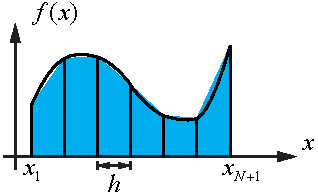
\includegraphics[width=6cm]{./figures/NumInt_1.pdf}
\caption{梯形法数值积分} \label{NumInt_fig1}
\end{figure}

接下来将每个区间的被曲线围出的面积用梯形来计算, 第 $i$ 个梯形面积为(两底和乘以高除以二)
$[f(x_{i+1}) + f(x_i)]h/2$. 定积分约等于所有梯形面积
\begin{equation}
\int_a^b f(x) \dd{x} \approx \sum_i^N  \frac h2 [f(x_{i+1}) + f(x_i)]
= h\qty[ \frac12 f(x_1) + \sum_{i = 2}^N f(x_i) + \frac12 f(x_{N+1})]
\end{equation}
显然, 当 $N$ 取越大时, 右边的求和就越接近定积分.

这里给出 Matlab 代码

\begin{lstlisting}[language=matlab, caption=trapezoidInt.m]
% 梯形法数值积分
% f 是被积函数的函数句柄
% [a, b] 为积分区间
% N 为子区间个数
function I = trapezoidInt(f, a, b, N)
x = linspace(a, b, N+1);
y = arrayfun(f, x); % 求所有 y(i) = f(x(i))
h = (b - a)/N;
I = h*(0.5*y(1) + 0.5*y(N+1) + sum(y(2:N)));
end
\end{lstlisting}

下面来看两个例子, 由算法可知, 当被积函数具有 $c_1 x + c_2$ 的形式时, 函数曲线围成的面积可由梯形精确解算, 所以即使 \verb|N| 取很小也可以精确到 \verb|double| 类型的精度(16 位左右).
\begin{lstlisting}[language=matlabC]
>> format long;
>> trapezoidInt(@(x)x, 0, 1, 4)
ans = 0.500000000000000
\end{lstlisting}
对其他一些函数, 需要较大的 $N$ 才能获得较高的精度. 我们已知 $\sin x$ 在 $[0, \pi]$ 内的积分等于 $2$, 再看数值积分
\begin{lstlisting}[language=matlabC]
>> trapezoidInt(@sin, 0, pi, 10)
ans = 1.983523537509455
>> trapezoidInt(@sin, 0, pi, 100)
ans = 1.999835503887444
>> trapezoidInt(@sin, 0, pi, 1000)
ans = 1.999998355065662
>> format short;
\end{lstlisting}
% 不难看出误差在 \order(1/N^2), 为什么呢?
